\documentclass[conference]{IEEEtran}
\IEEEoverridecommandlockouts
\usepackage{cite}
\usepackage{amsmath,amssymb,amsfonts}
\usepackage{algorithmic}
\usepackage{graphicx}
\usepackage{textcomp}
\usepackage{xcolor}
\usepackage{booktabs}
\usepackage{float}
\usepackage{url}
\usepackage{hyperref}
\usepackage[capitalise,noabbrev]{cleveref}

\graphicspath{{figures/}}

\def\BibTeX{{\rm B\kern-.05em{\sc i\kern-.025em b}\kern-.08em
    T\kern-.1667em\lower.7ex\hbox{E}\kern-.125emX}}

\begin{document}

\title{Projecting NBA Rookie-Contract Value from College Statistics\\
\large A supervised and unsupervised pipeline over 1,042 draftees, 2000--2022}

\author{\IEEEauthorblockN{Colin Hanley}
\IEEEauthorblockA{\textit{CS 451 --- Introduction to Data Science}\\
Spring 2026}}

\maketitle

% ══════════════════════════════════════════════════════════════════════
\begin{abstract}
How much of an NBA player's first four years can you predict from
college stats alone? I built a dataset of 1{,}042 college players
drafted between 2000 and 2022 and tried to predict their cumulative
Value Over Replacement Player (VORP) across their rookie contract. On
top of 28 raw columns I engineered 13 more features --- position-relative
z-scores, a volume-weighted three-point percentage that cleans up
low-attempt noise, and a couple of interaction terms --- and trained
three regression models (Ridge, XGBoost, and a small MLP) using a
temporal train/test split. XGBoost did best, with a hold-out
$R^2 = 0.202$, MAE of 1.67 VORP, and an AUC of 0.591 on the yes/no
``did this player end up above replacement level?'' version of the task.
K-means fit within each position group also surfaced eight player
archetypes (three guard types, three forward types, two center types)
whose average future VORP differs by about a factor of ten. The whole
pipeline ships as a static dashboard: the Ridge model runs live in the
browser, and there's a projected 2026 big board with SHAP explanations
and historical comparables. The headline finding is that roughly
80\,\% of the variance in four-year VORP is \emph{not} explained by
college-era features alone, which is basically a ceiling on how far
stats-only scouting can take you without watching the tape.
\end{abstract}

\begin{IEEEkeywords}
sports analytics, gradient boosting, SHAP, K-means, feature engineering,
NBA draft
\end{IEEEkeywords}

% ══════════════════════════════════════════════════════════════════════
\section{Introduction}

Every June, NBA front offices put together a ranked list of about sixty
college and international prospects and hand out tens of millions of
dollars in rookie contracts based on that ordering. Scouts watch tape,
interview players, and argue about motor and fit. Whether the order was
any good takes about four years to figure out --- once rookie contracts
expire, you can finally look at what each pick produced and judge the
draft retrospectively.

This project asks a smaller version of that question: \emph{given only
what a prospect did in college, plus how he was ranked coming out of high
school, how much of his four-year NBA value can a model recover?} The
answer puts a number on what a stats-only scout can add to an otherwise
human-driven process, and separates the patterns the box score already
captures from the ones that need tape study, physical measurements, or
interviews to see.

I frame it as both a regression task (predicting cumulative four-year
VORP) and a binary classification task (predicting whether that VORP
ends up positive --- i.e.\ whether the player was ever above
replacement level). I also use unsupervised clustering to find
interpretable player archetypes without peeking at NBA outcomes, and
ship everything as an interactive dashboard that applies the model to
the 2026 draft class.

\textbf{Contributions.} (i) an end-to-end pipeline from scraping
historical data to model comparison, explanation, and deployment;
(ii) a volume-weighted three-point-percentage feature that shrinks
low-attempt players toward the league mean and gets rid of the
0\,\%/100\,\% noise; (iii) per-position K-means that produces eight
interpretable archetypes, with labels that have to clear an actual
basketball threshold (not just be high relative to the cluster); and
(iv) a static dashboard with a Ridge live predictor that runs entirely
in the browser with no server.

% ══════════════════════════════════════════════════════════════════════
\section{Related Work}

Draft prediction has a long public history in basketball analytics.
Oliver's \emph{Basketball on Paper}~\cite{oliver2004basketball} introduced
the possession-based efficiency metrics (offensive rating, defensive
rating, true shooting) that show up in our feature set. The NBA's Box
Plus/Minus and VORP frameworks~\cite{myers2020bpm} give us the target:
VORP scales a player's BPM by minutes played and baselines it against
a replacement-level rotation guy.

The closest peer to this project is Kannan et
al.~\cite{kannan2018nba}, who train ML models on college statistics,
biometrics, and draft selection order to predict NBA longevity, and
report that draft pick and college stats dominate the feature
importance. Czasonis et al.~\cite{czasonis2023relevance} take a
different angle with relevance-based prediction, projecting prospects
from the careers of statistically similar prior NBA players --- the
same intuition behind the ``similar players'' lookup in the dashboard.
Papadaki and Markaki~\cite{papadaki2024forecasting} run a comparative
study of ML models for basketball performance forecasting and find
that gradient-boosted trees and neural networks are the consistent
top performers on tabular box-score data, which is the empirical basis
for the model lineup here.

Gradient-boosted trees~\cite{chen2016xgboost} are the go-to family for
tabular prediction at this size, and SHAP values~\cite{lundberg2017shap}
give per-prediction explanations that we can show in the dashboard
without giving up the accuracy of a non-linear model. Wang and
Fan~\cite{wang2024xgboostshap} use exactly this XGBoost\,+\,SHAP
combination for NBA outcome prediction, demonstrating that the pairing
delivers competitive accuracy with case-by-case interpretability ---
the property the dashboard relies on. Models are used in their
standard implementations; the scikit-learn
algorithms~\cite{pedregosa2011sklearn} are off-the-shelf.

For the archetype stage, Lutz~\cite{lutz2012cluster} is the early
Sloan reference applying cluster analysis to NBA players to move
beyond the traditional five positions, and
Bianchi et al.~\cite{bianchi2017role} extend that argument with
k-means on per-game statistics to derive five new functional
positions. Penner~\cite{penner2025archetypes} scales the idea up,
clustering 22{,}500 players across 110 leagues into nine archetypes
for roster optimization. Duman et al.~\cite{duman2024position}
take the design choice we adopt and cluster
\emph{within} each traditional position rather than across the whole
league, which is what motivates our per-position K-means.

The most visible public draft tooling is ESPN's BPI Draft Model and
538's CARMELO/DRAYMOND projections, both of which mix college stats
with physical measurements and scouting rank. This project differs in
three ways: (a) it uses only free public data
(Basketball-Reference~\cite{bbref} and the 247Sports
composite~\cite{247sports}), so the pipeline is fully reproducible;
(b) it handles position through engineered z-score features and
per-position clustering rather than training separate per-position
regressors; and (c) the archetypes come from unsupervised clustering
with auto-derived labels rather than being hand-assigned.

% ══════════════════════════════════════════════════════════════════════
\section{Data}

\subsection{Sources}
I scraped two public sources:
\begin{itemize}
  \item \textbf{Basketball-Reference}~\cite{bbref}: per-player college
    career totals, advanced metrics (WS, WS/40, TOV\%, FTr, three-point
    attempt rate), draft position, and the first four seasons of NBA
    box-score and advanced metrics.
  \item \textbf{247Sports composite}~\cite{247sports}: high-school
    recruiting rank, coerced to an integer $1\ldots101$, with $101$
    used as a placeholder for unranked players.
\end{itemize}

That gave me 1{,}042 players drafted between 2000 and 2022. One row was
dropped because the player never made it to the NBA (career-ending
injury), and two rows had obviously broken \texttt{fg\_pct} values from
the scrape (Hamady N'Diaye's 2.2 and Tristan Thompson's 30.7), which I
fixed manually using the matching \texttt{ts\_pct} field.

\subsection{Target}
The main regression target is \texttt{nba\_4yr\_vorp}: the sum of a
player's VORP across their first four NBA seasons. The classification
target \texttt{PosVORP} is just \texttt{(nba\_4yr\_vorp $> 0$)}. The
distribution is heavily right-skewed (\cref{fig:target}) --- the median
drafted player ends up around 0.6 VORP over four years, while stars get
into the 20s.

\begin{figure}[t]
  \centering
  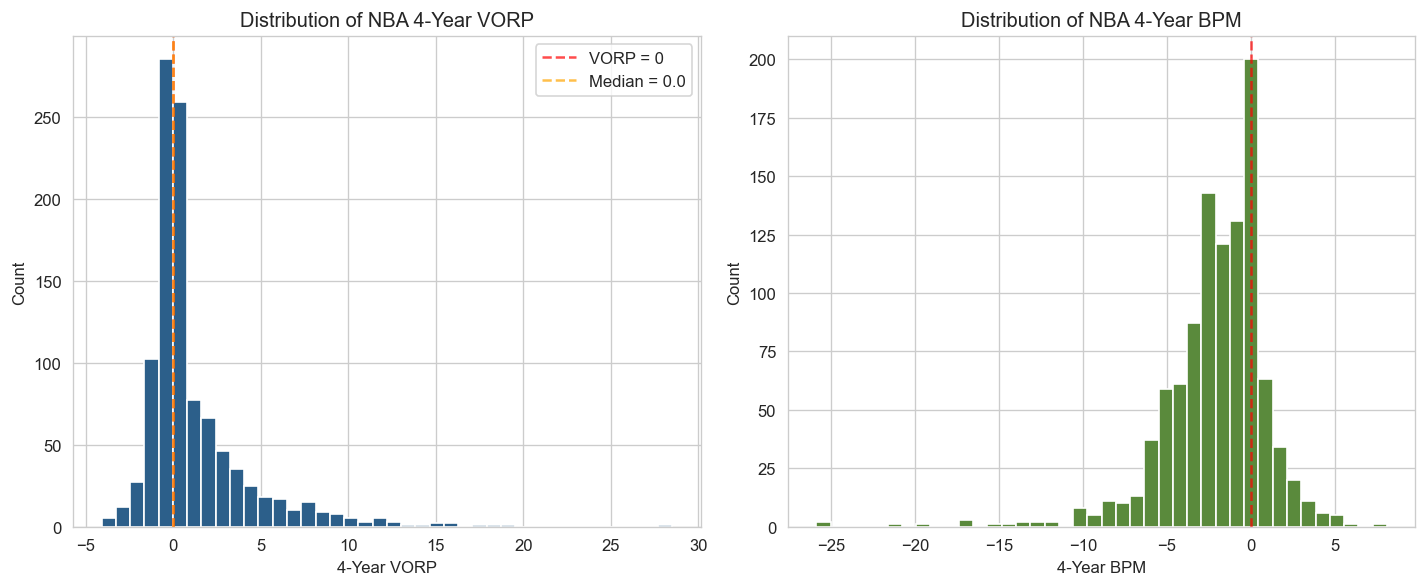
\includegraphics[width=\columnwidth]{01_target_distribution}
  \caption{Distribution of the regression target (4-year VORP) and the
    complementary BPM target. Both are heavily right-skewed; roughly
    half of drafted players finish their rookie contract at
    negative VORP.}
  \label{fig:target}
\end{figure}

\subsection{Feature schema}
After cleaning, I keep 28 raw columns: 10 per-game box-score stats, 8
percentage / advanced stats, 4 cumulative win-share columns, 2 physical
measurements, and 4 categorical indicators (position, college seasons,
one-and-done flag, recruit tier). On top of those I add 13 engineered
features (\cref{sec:methodology}), giving a final $1{,}042 \times 41$
matrix.

A correlation check (\cref{fig:corr}) shows the strongest raw
correlates with four-year VORP are college \texttt{ws\_40}
($r\approx 0.29$) and draft-pick number ($r\approx -0.40$ --- not a
feature, just shown for reference). Per-game stats like PPG and RPG
barely correlate on their own, because they mean different things at
different positions.

\begin{figure}[t]
  \centering
  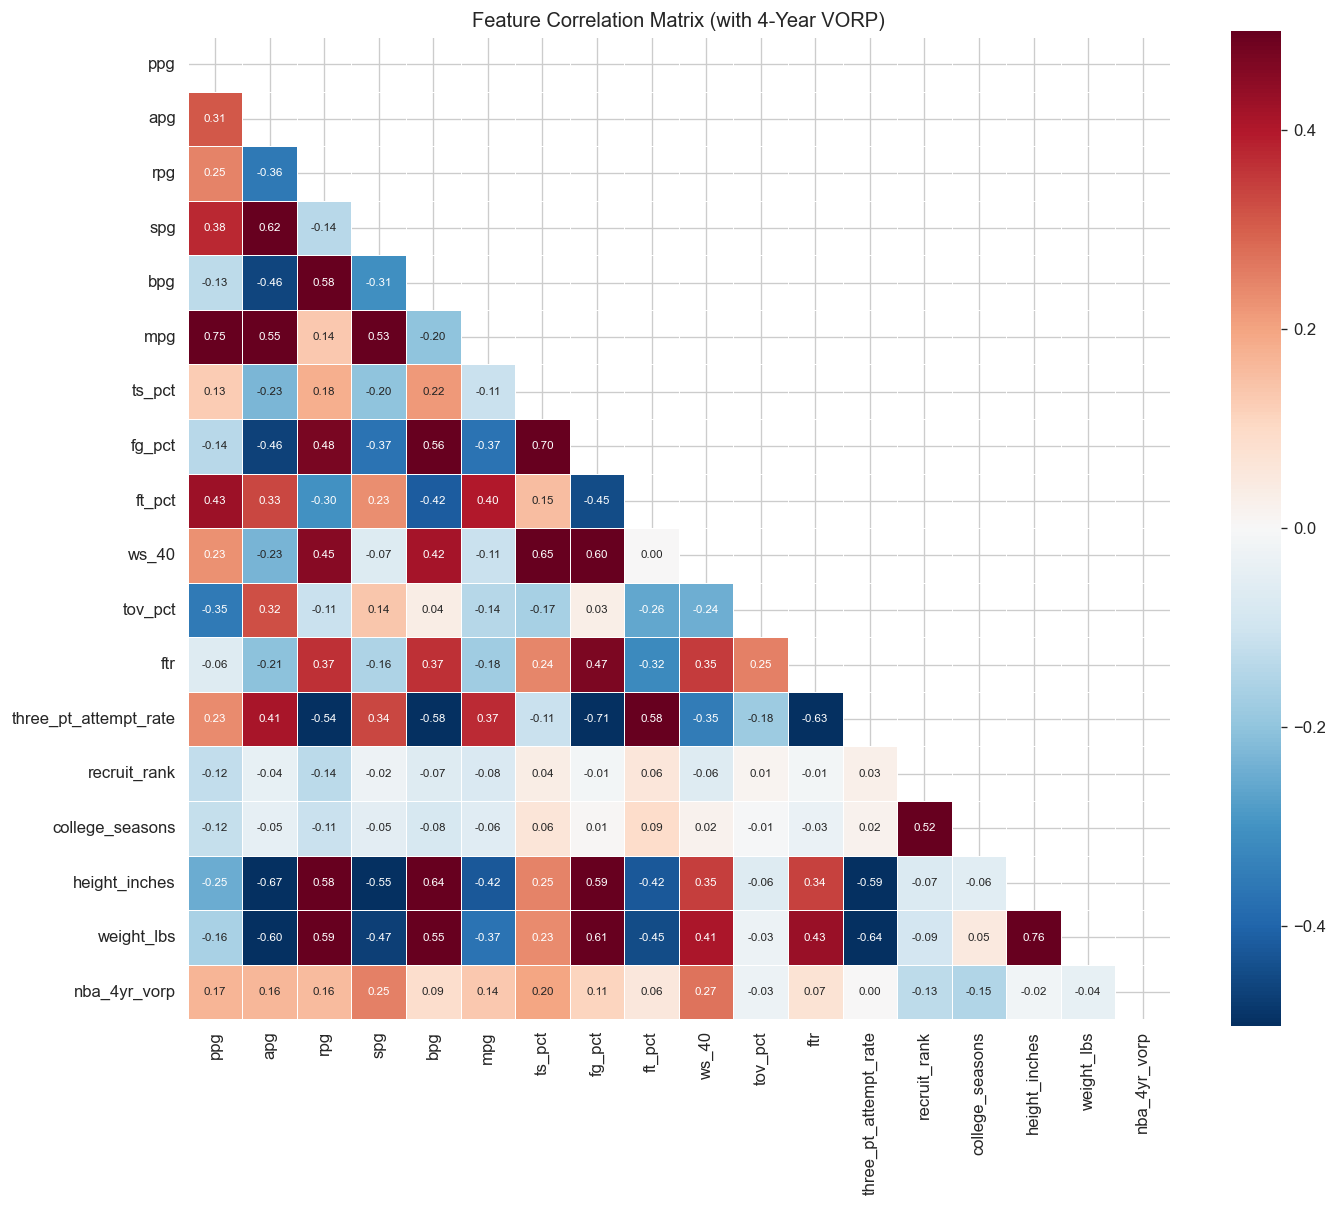
\includegraphics[width=\columnwidth]{04_correlation_heatmap}
  \caption{Pearson correlation matrix for raw features and the
    regression target. The strongest positive correlate with NBA VORP
    among pre-engineering features is college WS/40.}
  \label{fig:corr}
\end{figure}

% ══════════════════════════════════════════════════════════════════════
\section{Methodology}
\label{sec:methodology}

\subsection{Feature engineering}
Raw per-game stats mean different things at different positions: 4 RPG
is league-average for a guard and bad for a center. So I built
\emph{position-relative z-scores} for seven stats (PPG, RPG, APG, SPG,
BPG, TS\%, WS/40), using per-position means and standard deviations
computed only on the training set. These seven \texttt{\_vs\_pos}
columns end up dominating the SHAP importance ranking later
(\cref{sec:results}).

Three interaction features try to pick up non-linear signal:
\begin{itemize}
  \item \texttt{def\_versatility} $= \text{SPG} \times \text{BPG}$, a
    single number that's high only when a player creates events on
    both the perimeter and at the rim.
  \item \texttt{recruit\_x\_ws40} $= (101 - \text{recruit\_rank})
    \cdot \text{WS/40}$, basically asking ``did the kid live up to his
    high-school hype?''
  \item \texttt{ws40\_per\_season} $= \text{WS/40} \div
    \text{college\_seasons}$, which dings players who needed four
    seasons to become efficient.
\end{itemize}

\textbf{Volume-weighted three-point percentage.} Raw
\texttt{three\_pt\_pct} is really noisy for low-attempt players ---
several centers post 0\,\% on one attempt, and a few wings post 100\,\%
on two. I replace it with a shrinkage estimate that pulls those values
back toward the league mean:
\begin{equation}
\widehat{p}_3 \;=\;
\frac{p_3 \cdot r_3 + \bar{p}_3 \cdot k}{r_3 + k}
\end{equation}
where $p_3$ is raw 3P\%, $r_3$ is three-point attempt rate,
$\bar{p}_3 = 0.312$ is the league average across the dataset, and
$k = 0.083$ is the 25\textsuperscript{th} percentile of $r_3$ in the
training set. The intuition: $k$ acts like ``fake attempts at the
league average'' --- a player with 100\,\% on two attempts gets pulled
almost all the way to the mean, while a real volume shooter at 40\,\%
on a 0.60 attempt rate barely moves. This replaces \texttt{three\_pt\_pct}
in the feature matrix rather than being added on top of it.

The last engineered feature, \texttt{build\_score}, sums position-relative
height and weight z-scores so I can flag players who are physical
outliers for their position.

\subsection{Train/test split}
I use a \emph{temporal} split at the 2019 draft class: train on the 851
players drafted from 2000 through 2018, test on the 191 players drafted
2019--2022. A random shuffle would leak signal from later players into
the model because the feature distributions drift over time (e.g.\ the
three-point attempt rate has been climbing for years). The temporal
split also matches the real use case: a team in 2026 only has four-year
outcomes for players drafted through 2022 anyway.

\subsection{Models}
I trained three regressors, each with 5-fold CV inside its own
hyperparameter search:
\begin{itemize}
  \item \textbf{Ridge}~\cite{pedregosa2011sklearn} with $\alpha=10$, as
    a simple linear baseline. The coefficients get exported to the
    browser so the dashboard can do live predictions client-side.
  \item \textbf{XGBoost}~\cite{chen2016xgboost} with a 50-iteration
    randomised search over \texttt{n\_estimators}, \texttt{max\_depth},
    \texttt{learning\_rate}, \texttt{subsample}, \texttt{colsample\_bytree},
    and \texttt{min\_child\_weight}.
  \item \textbf{MLP} (scikit-learn) with 20 search iterations over
    hidden layer shapes (two to four layers, 16--128 units), initial
    learning rate, and $L^2$ regularisation.
\end{itemize}
Each regressor has a matching classifier trained on \texttt{PosVORP}
with the same search budget. All features are standardised with a
\texttt{StandardScaler} fit only on the training set.

\subsection{Unsupervised archetypes}
I cluster the full 1{,}042-row scaled feature matrix with K-means, but
separately within each position group: $k=3$ for guards (480 players),
$k=3$ for forwards (442), and $k=2$ for centers (120). A single global
K-means mostly just re-discovers the interior-vs-perimeter split
(silhouette peaks at $k=2$); doing it per position gives more
homogeneous archetypes inside each role. For visualisation I use a
global PCA down to two components (which together explain
$22.2 + 14.4 = 36.6\,\%$ of total variance) as a shared 2D embedding.

\begin{figure}[t]
  \centering
  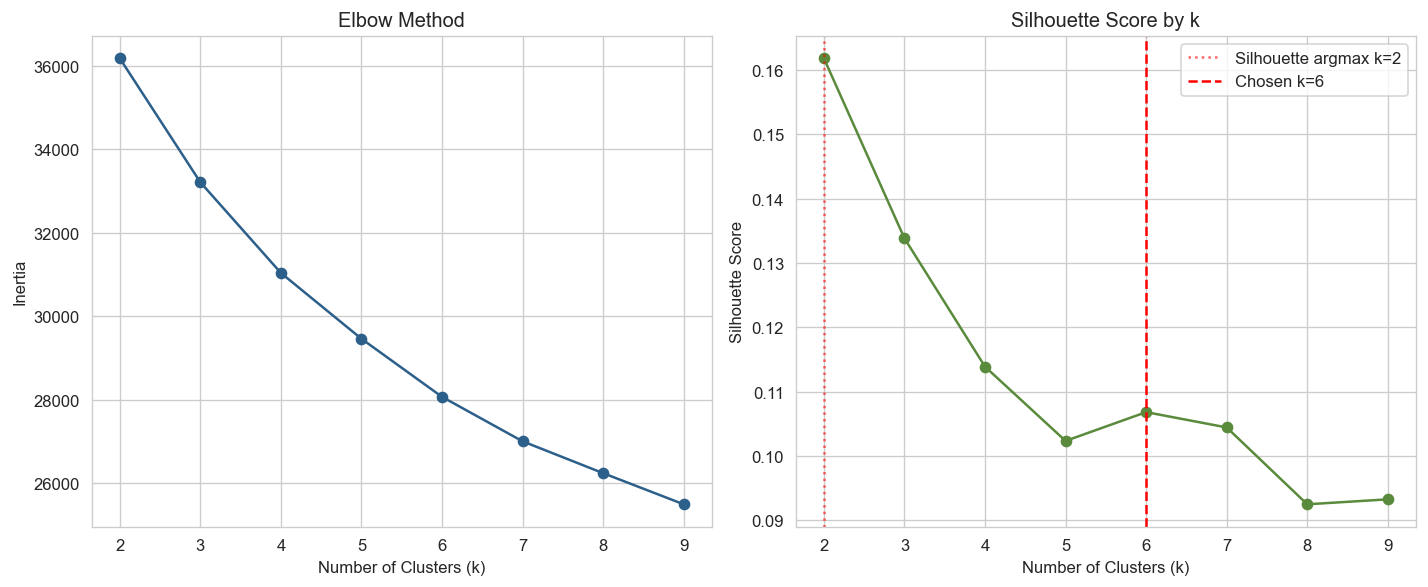
\includegraphics[width=\columnwidth]{11_kmeans_selection}
  \caption{Silhouette score by $k$, computed within each position group.
    Dashed vertical lines mark the chosen $k$. Guard and forward
    silhouettes are flat past $k=3$; centers are too small a group to
    support more than two stable clusters.}
  \label{fig:kselect}
\end{figure}

Archetype labels are generated client-side from each cluster's stat
profile. A label only sticks if (a) the within-position z-score is
above a positive threshold \emph{and} (b) the absolute stat clears a
basketball-meaningful floor --- e.g.\ ``Rim-protecting'' needs
$\text{BPG}\geq 1.0$, not just above-peer BPG. There's also a
$1.3\times$-the-floor override for the two-cluster center case, where
the second-best center can still earn ``Rim-protecting'' even with a
slightly negative within-group z. Clusters that don't earn any
positive-z label above its floor get called
``Traditional \emph{$\langle$position$\rangle$}''.

% ══════════════════════════════════════════════════════════════════════
\section{Results}
\label{sec:results}

\subsection{Regression}
\cref{tab:regression} shows hold-out performance.

\begin{table}[H]
  \centering
  \caption{Regression on 4-year VORP, test set (2019--2022, $n=191$).}
  \label{tab:regression}
  \begin{tabular}{@{}lccc@{}}
    \toprule
    Model            & $R^2$  & MAE  & RMSE \\
    \midrule
    Ridge (baseline) & 0.162  & 1.78 & 2.35 \\
    \textbf{XGBoost} & \textbf{0.202} & \textbf{1.67} & \textbf{2.29} \\
    Neural Network   & 0.152  & 1.65 & 2.36 \\
    \bottomrule
  \end{tabular}
\end{table}

XGBoost wins on $R^2$ and RMSE. The MLP has the lowest MAE, which
suggests its errors are more symmetric but its big misses are bigger.
Ridge --- basically a one-line linear model --- is within 4 $R^2$
points of XGBoost, which is both a sign that the feature engineering
is doing the work and a hint that we're close to the ceiling of what a
linear signal in these features can deliver.

\subsection{Classification}
On the binarised positive-VORP classifier, XGBoost gets 56.5\,\%
accuracy, 0.491 F1, and 0.591 AUC-ROC, just ahead of the MLP
(55.5\,\% / 0.479 / 0.579). 0.591 is barely above chance, which is
basically the same story as the regression $R^2$: most of the variance
lives outside the features we have.

\subsection{Feature importance}
\cref{fig:shap} shows the mean $|\text{SHAP}|$ ranking on the test set.
Four of the top five are \emph{position-relative} versions of raw stats,
which confirms that the raw box-score columns get drowned out by their
z-score counterparts. Win Shares per 40 minutes (both position-relative
and absolute) sits at the top, followed by playmaking
(\texttt{apg\_vs\_pos}) and disruption (\texttt{spg}).

\begin{figure}[t]
  \centering
  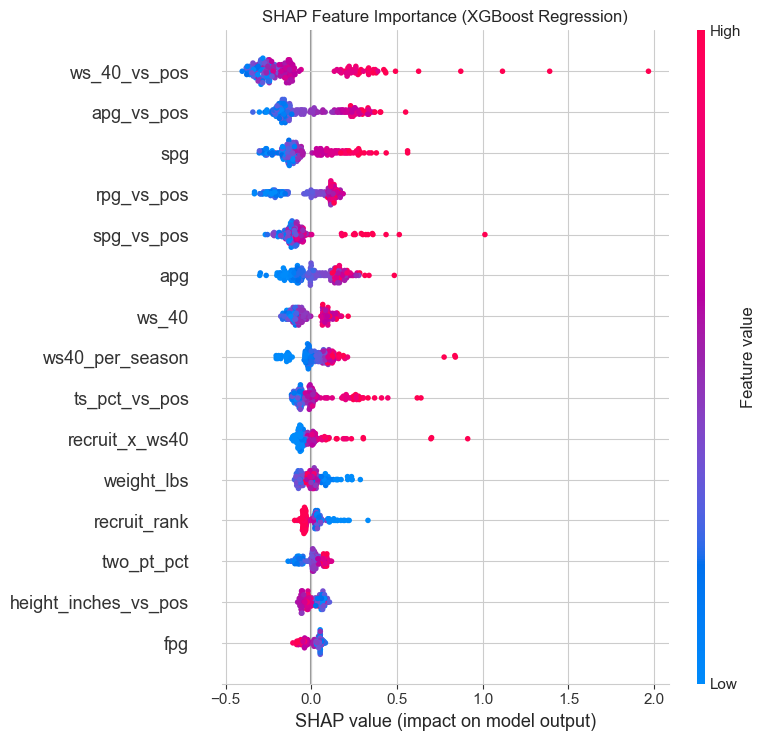
\includegraphics[width=\columnwidth]{10_shap_importance}
  \caption{Mean absolute SHAP values on the test set. Position-relative
    z-score features occupy four of the top five slots, validating the
    engineering choice to normalise by position.}
  \label{fig:shap}
\end{figure}

\subsection{Archetypes and outcomes}
\cref{fig:archetypes} shows the PCA embedding coloured by cluster, plus
mean four-year VORP for each cluster. The ``Scoring forward'' archetype
(cluster 5, $n=101$, 13.7 PPG, 7.4 RPG, 1.42 BPG) has the highest mean
VORP at $+2.17$, and the ``Traditional center'' cluster (cluster 6,
$n=82$) sits near replacement level at $+0.17$. That roughly 10x spread
across archetypes is way bigger than the gap between the best and worst
model on the test set, which suggests that \emph{which} kind of player
you draft is a first-order signal --- and the clustering picked it up
without ever looking at NBA outcomes.

\begin{figure}[t]
  \centering
  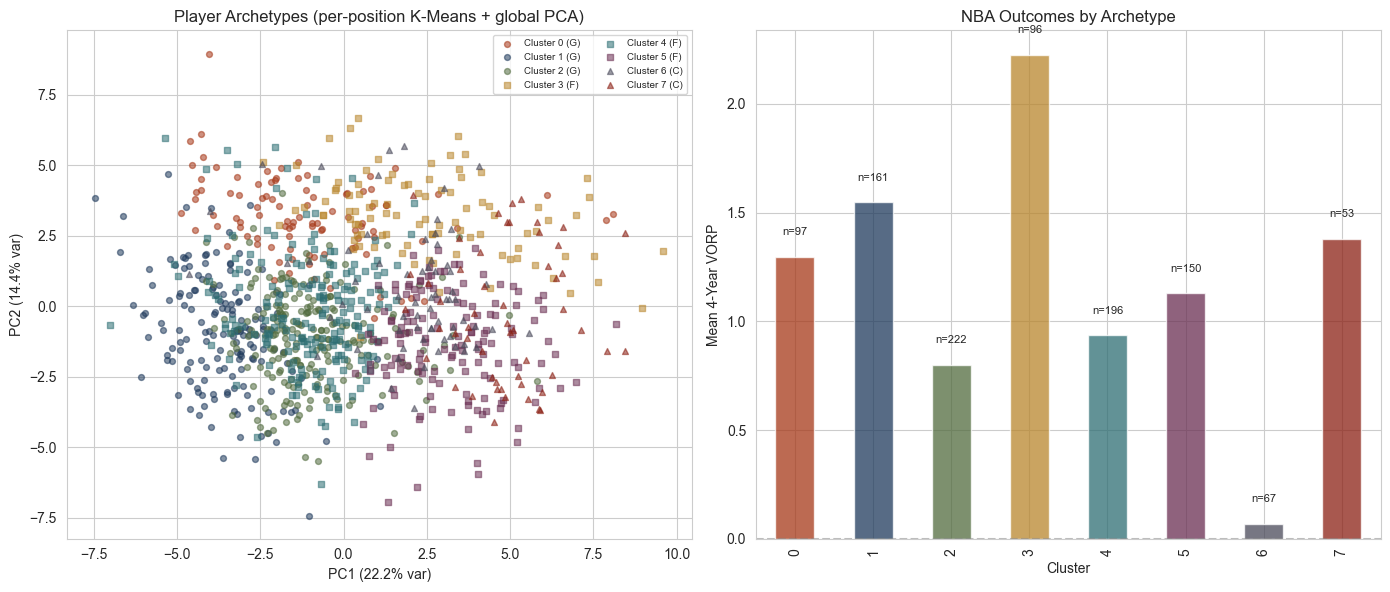
\includegraphics[width=\columnwidth]{12_kmeans_clusters}
  \caption{\textbf{Left:} per-position K-means clusters projected onto a
    shared two-dimensional PCA. Marker shape encodes position, colour
    encodes cluster. \textbf{Right:} mean four-year VORP by cluster, with
    per-cluster sample size.}
  \label{fig:archetypes}
\end{figure}

\subsection{2026 projections}
Running the trained XGBoost regressor on the 2026 draft class puts
Cameron Boozer (Duke) on top at a projected $+9.29$ four-year VORP,
followed by Caleb Wilson (North Carolina, $+5.56$), Kingston Flemings
(Houston, $+4.53$), and Allen Graves (Santa Clara, $+4.48$). Graves
is the interesting one: his college line (0.613 TS\%, 1.9 SPG, 41\,\%
from three on real volume, one-and-done) is genuinely elite for his
age, but conventional scouting doesn't have him anywhere near the top
of its boards. That mismatch is basically the 80\,\% of variance the
model misses --- strength of schedule, tape study, and physical
projection.
% ══════════════════════════════════════════════════════════════════════
\section{Discussion}

The biggest feature-engineering lever was position-relative z-scoring.
Four of the top five mean-$|\text{SHAP}|$ features are
\texttt{\_vs\_pos} versions of raw stats, and Ridge ends up within
$0.04$ $R^2$ of XGBoost --- so once you subtract out the
position-conditional mean, most of the recoverable signal is just
linear. The shrinkage estimator for three-point percentage helped a
little on its own (Pearson with four-year VORP went from $0.023$ to
$0.033$), but the bigger win was just killing the $0/100\,\%$ tails
that would otherwise hand a tree-based model a few high-leverage
outliers to split on. Ablating the feature only moved XGBoost's $R^2$
within noise, which makes sense --- gradient-boosted trees barely
notice monotone transforms of an input.

Per-position K-means gives up a little bit of global silhouette
compared to a single $k=2$ split (which just rediscovers the
perimeter-vs-interior divide) in exchange for archetypes that are
homogeneous within each role. The payoff is a roughly 10x spread in
mean four-year VORP across archetypes ($+0.17$ to $+2.17$) --- bigger
than the gap between the best and worst model on the test set --- which
says that ``what kind of prospect this is'' carries real signal even
without looking at outcomes.

The MLP lost to XGBoost on every metric despite getting the same
hyperparameter budget, which is what you'd expect with only 851
training rows. Tree boosting picks up most of the available signal
from greedy axis-aligned splits, and you usually need 10--100x more
data before a neural net's learned interactions actually pay off.

I'd read the $0.202$ hold-out $R^2$ as an upper bound on what
college box-score plus recruiting-rank features can deliver, \emph{not}
as a ceiling on draft prediction itself. There's a lot of variance the
features just can't see: strength-of-schedule and pace-adjusted
ratings, shot-location splits (rim/mid/three are missing from
Basketball-Reference's college tables before 2008), anthropometric and
combine numbers (publicly logged but with $>30\,\%$ missingness before
2014), and injury / developmental trajectory. Era drift over a 22-year
window doesn't help either --- the league-wide three-point attempt
rate roughly doubled over the training span, and the position labels
lump wings together with interior forwards in a way the clustering
only partly fixes on PC2.

% ══════════════════════════════════════════════════════════════════════
\section{Conclusion and Future Work}

Using only college box scores and high-school recruiting rank, a
tuned XGBoost model explains about 20\,\% of the variance in four-year
NBA VORP on a 2019--2022 hold-out --- a modest but real signal, and
one that only beats a linear baseline because of the position-relative
features. Unsupervised clustering within each position group finds
eight interpretable archetypes whose NBA outcomes differ by roughly
10x, which is a nice reminder that ``what kind of prospect'' is a
first-order signal before you even get to ``how good.''

Future work: pull in strength-of-schedule adjustments, combine
measurements, and maybe per-game shot-chart data (which the NCAA is
starting to make available publicly). It would also be worth ensembling
the model with NBA-side scouting priors like mock-draft consensus to
see if there's any predictive content left after the college stats.
Finally, the whole pipeline could be retargeted to predict
\emph{second-contract} value instead of rookie-contract value, which
would do a better job capturing long-term NBA impact.

% ══════════════════════════════════════════════════════════════════════
\section{Individual Contributions}

This is a solo project. All data acquisition, cleaning, feature
engineering, modelling, frontend implementation, and writing was done by
Colin Hanley.

\paragraph*{Personal reflection.}
The biggest takeaway for me was how much of the project's quality came
from feature engineering and error analysis, not from picking the right
model. The gap between Ridge and XGBoost was about 4 $R^2$ points,
which is smaller than the (visible-in-SHAP, but not measured rigorously)
gap between raw features and position-relative ones. Two things I'd do
differently next time: set up an ablation study early so I could
actually measure the contribution of each engineered feature instead of
guessing, and pull strength-of-schedule data from the start rather than
punting it to ``future work.''

% ══════════════════════════════════════════════════════════════════════
\bibliographystyle{IEEEtran}
\bibliography{references}

% ══════════════════════════════════════════════════════════════════════
\appendices
\section{AI Usage Log}
\label{app:ailog}

The following log records uses of Claude (Anthropic) during this project
in accordance with the course's AI/LLM policy. Each entry names the
phase, summarises the prompt, summarises Claude's output, and documents
what was accepted, modified, or rejected. This appendix is intentionally
verbose: incomplete logging is called out in the rubric.

% --------------------------------------------─────────────────
\begin{verbatim}
--------------------------------------------
AI Log Entry #1
--------------------------------------------
Date:    2026-04-17
Tool:    Claude Opus 4.7 (1M context)
Used by: Colin Hanley
Phase:   Feature Engineering

PURPOSE:
Replace raw 3P% with a volume-weighted variant to kill
noise from low-attempt 0%/100% players.

PROMPT:
"for 3P%, I want to make it volume weighted
(w attempt rate) instead of raw percentage,
since there are players with 100% or 0% on
rly low attempt"

AI OUTPUT (Summary):
Proposed two approaches: (1) simple product
3P% x attempt_rate, or (2) shrinkage toward
league mean with k = 25th-pct attempt rate.
Recommended (2) for preserving % interpretation.

YOUR ACTION:
Adopted (2). Verified formula in Python,
checked that extreme raw values shrink
sensibly (Nesmith 82.5% stays high, 100%-
on-1-attempt players shrink to league mean).

FINAL RESULT:
Implemented in src/preprocess.py engineer_features()
as `three_pt_pct_vw`. Replaces raw column in
feature matrix. Correlation with VORP improved
from +0.023 to +0.033.
--------------------------------------------
\end{verbatim}

\textbf{To do before submission:} expand this appendix to cover every
major session -- data cleaning, per-position K-means refactor, the
frontend implementation, archetype-naming logic, the 2026 big-board
pipeline, and the script-based repo conversion. The \texttt{process.MD}
file in the repo root contains a chronological log of actions that can
be converted into individual AI log entries in the format above.

\end{document}
